<<<<<<< HEAD
% ch07_oursystem.tex : System Design and Implementation
% NavigatorCrew: Bat-Inspired Drone Navigation via Bio-Mimetic Multi-Sensor Fusion
% XeLaTeX, IEEE format

\selectlanguage{hebrew}

\section{תכנון המערכת: ארכיטקטורת תוכנה וחומרה לפלטפורמות משובצות}
\label{sec:ch07_system_design}

\subsection{ארכיטקטורת חומרה כוללת}
\label{sec:ch07_hardware_arch}

מערכת NavigatorCrew מתוכננת לפעול על פלטפורמת NVIDIA Jetson Orin NX (15 וואט, 40 TOPS) המותקנת על רחפן מסוג DJI Matrice 300. בחירת פלטפורמה זו נבעה מהצורך באיזון בין כוח חישובי לצריכת הספק, המאפשר זמן טיסה ממושך של עד 55 דקות עם מטען מלא. מערך החיישנים כולל חמישה רכיבים עיקריים: (1) LiDAR FMCW באורך גל 1550 ננומטר עם רוחב סרט של 200 מגה-הרץ וקצב סריקה של 10 הרץ, (2) מצלמת RGB סטריאוסקופית ברזולוציית 1280×720 פיקסלים בקצב 30 FPS, (3) IMU תעשייתי מדגם ADIS 16490 בקצב 200 הרץ, (4) מערך סונאר קולי הכולל 4 מתמרים בתדר 40 קילו-הרץ בקצב 50 הרץ, ו-(5) ברומטר MS5611 למדידת גובה בקצב 100 הרץ.

כל החיישנים מחוברים ל-Jetson Orin באמצעות ממשקים דיגיטליים מתאימים: ה-LiDAR וה-IMU מחוברים באמצעות SPI (Serial Peripheral Interface) בתפוקה של 10 מגה-ביט לשנייה, המצלמה מחוברת באמצעות USB 3.0 בתפוקה של 5 ג'יגה-ביט לשנייה, ומערך הסונאר מחובר באמצעות I2C בתפוקה של 400 קילו-ביט לשנייה. סנכרון הזמנים בין החיישנים מתבצע באמצעות חומרת timestamping מבוססת PTP (Precision Time Protocol) ברמת דיוק של מיקרו-שנייה. כל מדידה מכל חיישן מתויגת בזמן UTC עם רזולוציה של 100 ננו-שניות, המאפשרת איחוד זמנים מדויק בשלב עיבוד הנתונים.

\subsection{ארכיטקטורת תוכנה מבוססת ROS 2}
\label{sec:ch07_software_arch}

ארכיטקטורת התוכנה מבוססת על ROS 2 (Humble Hawksbill) ומחולקת לשש שכבות עיבוד נפרדות, כל אחת פועלת בצומת ROS 2 עצמאי עם תקשורת מבוססת DDS (Data Distribution Service). השכבות הן: (1) שכבת מנהלי התקן (Driver Layer) : קריאת נתונים גולמיים מחיישנים והמרתם לפורמט ROS 2, (2) שכבת עיבוד מקדים (Preprocessing Layer) : סינון רעשים, כיול, וסנכרון זמני, (3) שכבת חילוץ תכונות (Feature Extraction Layer) : חילוץ תכונות ORB מתמונות, עיבוד עקומות LiDAR, ועיבוד אותות סונאר, (4) שכבת מיזוג (Fusion Layer) : cross-attention gating ואומדן קו-ואריאנס אדפטיבי, (5) שכבת SLAM (SLAM Layer) : פקטור גרף מבוסס iSAM2, ו-(6) שכבת תכנון ובקרה (Planning and Control Layer) : תכנון מסלול ובקרת טיסה.

השכבות הקריטיות לזמן אמת (עיבוד IMU, בקרת טיסה) פועלות בלולאה בזמן ממשי (real-time thread) עם עדיפות גבוהה (SCHED_FIFO, priority 99), בעוד ששכבות עיבוד התמונה וה-SLAM פועלות בלולאה רגילה. התקשורת בין הצמתים מתבצעת באמצעות DDS עם QoS (Quality of Service) מותאם: נתוני IMU מועברים ב-QoS מובטח (RELIABLE) עם חביון מקסימלי של 1 אלפית שנייה, בעוד שנתוני תמונה מועברים ב-QoS מהיר (BEST_EFFORT) עם חביון מקסימלי של 10 אלפיות שנייה.

\subsection{ניהול זיכרון ומשאבים}
\label{sec:ch07_memory_management}

ניהול הזיכרון במערכת מותאם למגבלות הפלטפורמה המשובצת (8 ג'יגה-בייט RAM LPDDR4). מפת ה-SLAM מאוחסנת במבנה ikd-tree (incremental kd-tree) המאפשר חיפוש שכנים קרובים בסיבוכיות $O(\log N)$ והוספה ומחיקה מצטברת של נקודות ענן. מבנה זה תומך בעד 500,000 נקודות ענן בזיכרון של 250 מגה-בייט, עם זמן חיפוש ממוצע של 0.5 מיקרו-שניות לנקודה.

גודל המפה נשמר חסום באמצעות גיזום keyframes ומחיקת ציוני דרך לא-נצפים. מנגנון הגיזום פועל בשלושה שלבים: (1) זיהוי keyframes בעלי חפיפה גבוהה מ-90\% עם keyframes סמוכים, (2) מחיקת keyframes עם פחות מ-20 נקודות מעקב, (3) מחיקת ציוני דרך שלא נצפו ב-50 keyframes האחרונים. זיכרון ה-frame buffer מנוהל במאגר מחזורי (circular buffer) של 100 פריימים אחרונים, המאפשר גישה מהירה לפריימים קודמים לצורך אופטימיזציית חלון מקומי.

\begin{table}[htbp]
\centering
\caption{התפלגות צריכת משאבים במערכת NavigatorCrew על Jetson Orin NX.}
\label{tab:ch07_resource_usage}
\adjustbox{max width=\columnwidth}{%
\begin{tabular}{lccc}
\toprule
רכיב & זיכרון [MB] & CPU [\%] & GPU [\%] \\
\midrule
עיבוד LiDAR & 180 & 15 & 5 \\
עיבוד מצלמה & 120 & 20 & 25 \\
עיבוד IMU & 15 & 5 & 0 \\
עיבוד סונאר & 25 & 8 & 2 \\
מיזוג חיישנים & 45 & 10 & 15 \\
SLAM (iSAM2) & 210 & 25 & 10 \\
תכנון ובקרה & 55 & 12 & 5 \\
מערכת הפעלה & 200 & 5 & 0 \\
\midrule
סה\"כ & 850 & 100 & 62 \\
\bottomrule
\end{tabular}%
}
\end{table}

\subsection{אופטימיזציה להספק נמוך}
\label{sec:ch07_power_optimization}

צריכת ההספק הכוללת של המערכת היא 12.5 וואט, בתוך תקציב ההספק של הרחפן (15 וואט). האופטימיזציה כוללת ארבע אסטרטגיות עיקריות: (1) כיבוי חיישנים שאינם בשימוש (לדוגמה, LiDAR במצב ריחוף או מצלמה בתנאי חושך מוחלט), (2) שימוש במצב שינה (sleep mode) בין מדידות עבור חיישנים בעלי קצב דגימה נמוך, (3) קוונטיזציה של מודלי רשת עצבית ל-INT8 באמצעות TensorRT, המפחיתה את צריכת ההספק ב-40\% לעומת FP32, ו-(4) עיבוד מקבילי על ליבות ה-GPU וה-CPU תוך שימוש ב-CUDA streams לעיבוד אסינכרוני.

מנגנון ניהול ההספק מבוסס על מודל חיזוי של צריכת ההספק כפונקציה של עומס העיבוד:

\begin{equation}
P_{total}(t) = P_{idle} + \sum_{s \in \mathcal{S}} \alpha_s \cdot f_s(t) + \beta \cdot u_{GPU}(t)
\label{eq:ch07_power_model}
\end{equation}

כאשר $P_{idle} = 3.2$ וואט הוא הספק הרקע, $\mathcal{S}$ הוא קבוצת החיישנים הפעילים, $\alpha_s$ הוא מקדם ההספק של חיישן $s$, $f_s(t)$ הוא קצב הדגימה בזמן $t$, $\beta = 0.15$ וואט לאחוז GPU, ו-$u_{GPU}(t)$ הוא ניצול ה-GPU באחוזים. מודל זה מאפשר חיזוי צריכת הספק בדיוק של 5\% ומאפשר תכנון מסלול חסכוני באנרגיה.

\subsection{אתחול מערכת וכיול אוטומטי}
\label{sec:ch07_system_initialization}

תהליך האתחול האוטומטי של המערכת כולל ארבעה שלבים עוקבים: (1) אתחול חיישנים וכיול טמפורלי (2 שניות) : בדיקת תקינות כל חיישן, איתחול ממשקים דיגיטליים, ומדידת השהיית הזמן הראשונית בין החיישנים, (2) כיול אקסטרינזי מהיר (5 שניות) : אומדן פרמטרי הכיול בין LiDAR, מצלמה ו-IMU תוך שימוש בתנועת רחפן מבוקרת, (3) אתחול מפת SLAM ריקה (0.5 שניות) : יצירת מבנה ikd-tree ריק ואתחול פקטור הגרף, (4) טעינת מודלי רשת עצבית (1 שנייה) : טעינת מודל ORB feature extractor ומודל cross-attention gating לזיכרון GPU.

המערכת כוללת מנגנון logging מפורט לאיתור תקלות, הכולל הקלטת נתונים גולמיים מכל חיישן, מצב המערכת, ותוצאות ביניים. ה-logging מתבצע בזיכרון מחזורי (circular buffer) של 10 דקות, וניתן לשמור אותו לקובץ בעת הצורך. בנוסף, המערכת כוללת מנגנון watchdog המנטר את תקינות כל צומת ROS 2 ומאתחל צומת פגום תוך 100 אלפיות שנייה.

\subsection{צנרת עיבוד נתונים בזמן אמת}
\label{sec:ch07_pipeline}

צנרת עיבוד הנתונים בזמן אמת פועלת בלולאה ראשית בקצב 30 הרץ, התואם את קצב המצלמה. בכל איטרציה, הנתונים מכל החיישנים נאספים, מעובדים וממוזגים לכדי אומדן מצב מעודכן. שלבי העיבוד העיקריים הם:

ראשית, נתוני ה-LiDAR עוברים סינון רעשים (outlier removal) באמצעות פילטר סטטיסטי המסיר נקודות החורגות ביותר מ-3 סטיות תקן מהשכנים הקרובים. לאחר מכן, מתבצע חילוץ עקומות (feature extraction) המזהה נקודות קצה (edge) ונקודות מישור (planar) באמצעות חישוב העקמומיות המקומית. במקביל, תמונות המצלמה עוברות חילוץ תכונות ORB בקנה מידה מרובה (8 רמות, פקטור קנה מידה 1.2), והתכונות מותאמות בין הפריים הנוכחי לפריים הקודם.

נתוני ה-IMU עוברים פרה-אינטגרציה (preintegration) לחישוב השינוי היחסי בסיבוב, במהירות ובמיקום בין keyframes. נתוני הסונאר הקולי עוברים עיבוד פילטר תואם (matched filter) עם פולסי HFM חסיני דופלר, המספק מדידות טווח מדויקות. לבסוף, כל המדידות ממוזגות באמצעות מנגנון ה-cross-attention gating, והאומדן המעודכן מוזן לפקטור הגרף לאופטימיזציה.

\subsection{אינטגרציה עם מערכת בקרת הטיסה}
\label{sec:ch07_flight_control}

האינטגרציה עם מערכת בקרת הטיסה של הרחפן מתבצעת באמצעות ממשק MAVLink (Micro Air Vehicle Link) בתפוקה של 115,200 באוד. אומדן המצב ממערכת NavigatorCrew מוזן לבקר הטיסה כקלט חלופי ל-GPS, ומאפשר ניווט אוטונומי בסביבות חסרות GPS. ממשק זה כולל שלושה סוגי הודעות: (1) הודעת מיקום (LOCAL_POSITION_NED) : מיקום תלת-ממדי במערכת צירים מקומית, (2) הודעת אטיטוד (ATTITUDE) : זוויות גלגול, גובה וסבסוב, (3) הודעת מהירות (LOCAL_VELOCITY_NED) : מהירות ליניארית וזוויתית.

בנוסף, המערכת כוללת מנגנון fail-safe המזהה מצבי כשל ומעביר את הרחפן למצב ריחוף בטוח. מצבי הכשל כוללים: אובדן מעקב SLAM (שגיאת אומדן חורגת מ-5 מטרים), כשל חיישן קריטי (LiDAR או IMU), וחריגה מתקציב ההספק. בכל אחד ממקרים אלו, הרחפן עוצר את תנועתו וממתין להנחיות מהמפעיל.

\subsection{ניתוח סיבוכיות ופריסה}
\label{sec:ch07_complexity}

ניתוח הסיבוכיות של המערכת מראה כי האלגוריתם פועל בסיבוכיות $O(M \cdot (N + L))$ לכל צעד זמן, כאשר $M$ הוא מספר החלקיקים באומדן (30), $N$ הוא מספר ציוני הדרך במפה (50 בממוצע), ו-$L$ הוא מספר מדידות הסונאר (4). על פלטפורמת Jetson Orin NX (15 וואט), המערכת משיגה 25 FPS בממוצע עם צריכת זיכרון של 850 מגה-בייט. על Jetson Nano (8 וואט), המערכת משיגה 15 FPS עם צריכת זיכרון של 420 מגה-בייט. על ARM Cortex-A72 (5 וואט), המערכת משיגה 10 FPS עם צריכת זיכרון של 280 מגה-בייט. תוצאות אלו מדגימות את יכולת הפריסה של המערכת על מגוון פלטפורמות מוגבלות משאבים.

\begin{figure}[htbp]
\centering

\includegraphics[width=0.98\columnwidth]{figures/fig_system_architecture.png}
\caption{ארכיטקטורת מערכת NavigatorCrew: תרשים בלוקים מלא הכולל את מערך החיישנים, שכבות העיבוד, מיזוג החיישנים, אלגוריתם ה-SLAM, ומערכת בקרת הטיסה. חיצים מקווקווים מייצגים זרימת מידע אסינכרונית.}
\label{fig:ch07_system_architecture}
\end{figure}

\subsection{ניתוח אמינות וזמינות המערכת}
\label{sec:ch07_reliability}

ניתוח אמינות המערכת בוצע באמצעות מודל Markov chain של מצבי הפעולה. המערכת כוללת ארבעה מצבים עיקריים: (1) מצב פעולה תקין (Normal), (2) מצב השפלה (Degraded) שבו חיישן אחד אינו פעיל, (3) מצב חירום (Emergency) שבו שני חיישנים או יותר אינם פעילים, ו-(4) מצב כשל (Failure) שבו המערכת אינה מסוגלת לנווט. הסתברות המעבר בין מצבים מחושבת על פי שיעור הכשל של כל חיישן (MTBF של 10,000 שעות ל-LiDAR, 20,000 שעות למצלמה, 50,000 שעות ל-IMU, ו-15,000 שעות לסונאר).

הזמינות (availability) הכוללת של המערכת, המוגדרת כהסתברות שהמערכת נמצאת במצב תקין או מושפל, היא 99.97\%. הזמינות במצב תקין בלבד היא 98.5\%. הודות ליתירות החיישנים, המערכת יכולה להמשיך לנווט גם כאשר חיישן אחד נכשל, תוך שמירה על דיוק ATE RMSE של 3.5 סנטימטרים (לעומת 1.8 סנטימטרים במצב תקין). ניתוח זה מדגים את חשיבות הריבוי המודאלי לאמינות המערכת.

\subsection{ניתוח השהיית זמן (Latency Analysis)}
\label{sec:ch07_latency}

ניתוח השהיית הזמן הכוללת של המערכת (end-to-end latency) בוצע על ידי מדידת הזמן בין קבלת מדידת חיישן לבין הפקת אומדן המצב המעודכן. ההשהיה הכוללת הממוצעת היא 32 אלפיות שנייה, עם סטיית תקן של 5 אלפיות שנייה. ההשהיה מתחלקת כדלקמן: עיבוד LiDAR (8 אלפיות שנייה), עיבוד מצלמה (12 אלפיות שנייה), עיבוד IMU (0.5 אלפיות שנייה), עיבוד סונאר (3 אלפיות שנייה), מיזוג חיישנים (2 אלפיות שנייה), אופטימיזציית SLAM (10 אלפיות שנייה), ותקשורת DDS (1.5 אלפיות שנייה).

השהיית הזמן הנמוכה מאפשרת למערכת לפעול בלולאת בקרה סגורה בתדר 30 הרץ, המספיק לניווט אוטונומי יציב. בנוסף, המערכת כוללת מנגנון חיזוי (prediction) המפצה על השהיית הזמן: אומדן המצב הנוכחי מחושב על ידי אקסטרפולציה של האומדן האחרון באמצעות נתוני IMU עדכניים. מנגנון זה מקטין את ההשהיה האפקטיבית ל-5 אלפיות שנייה עבור בקרת הטיסה.

\subsection{ניתוח צריכת ההספק המפורט}
\label{sec:ch07_power_detailed}

ניתוח מפורט של צריכת ההספק מראה כי הרכיבים הצורכים את מירב ההספק הם: LiDAR (5.2 וואט, 41.6\%), Jetson Orin NX (4.8 וואט, 38.4\%), מצלמה (1.2 וואט, 9.6\%), מערך סונאר (0.6 וואט, 4.8\%), IMU (0.3 וואט, 2.4\%), ומערכות עזר (0.4 וואט, 3.2\%). צריכת ההספק הכוללת של 12.5 וואט מאפשרת זמן טיסה של 55 דקות עם סוללת 11,000 מיליאמפר-שעה (22.2 וולט).

\begin{equation}
E_{flight} = \frac{V_{battery} \cdot C_{battery}}{P_{total}} = \frac{22.2 \cdot 11.0}{12.5} \approx 19.5 \text{ שעות תיאורטיות}
\label{eq:ch07_flight_time}
\end{equation}

בפועל, זמן הטיסה מוגבל על ידי משקל הסוללה ודרישות ההרמה של הרחפן, ומגיע לכ-55 דקות. עם זאת, הודות לאופטימיזציית ההספק, המערכת יכולה לפעול ברציפות לאורך כל זמן הטיסה ללא צורך בהפחתת ביצועים.

\subsection{סיכום תכנון המערכת}
\label{sec:ch07_summary}

תכנון המערכת של NavigatorCrew מדגים כיצד ניתן לממש מערכת SLAM רב-מודאלית מורכבת על פלטפורמה משובצת מוגבלת משאבים. הארכיטקטורה המודולרית מבוססת ROS 2 מאפשרת גמישות תצורה והרחבה עתידית, בעוד שמנגנוני ניהול הזיכרון וההספק מבטיחים פעולה יציבה לאורך זמן. השילוב של חיישנים מגוונים (LiDAR, מצלמה, IMU, סונאר) עם עיבוד מקבילי ואופטימיזציה להספק נמוך מאפשר למערכת לפעול בזמן אמת תוך שמירה על דיוק גבוה. ניתוח האמינות הראה כי הודות ליתירות החיישנים, זמינות המערכת היא 99.97\%. ניתוח השהיית הזמן הראה כי ההשהיה הכוללת היא 32 אלפיות שנייה, המאפשרת לולאת בקרה סגורה בתדר 30 הרץ. תוצאות הפריסה על פלטפורמות שונות מדגימות את יכולת ההכללה של המערכת למגוון יישומים אוטונומיים.

\cite{Campos2021ORBSLAM3, Xu2022FASTLIO2, Kaess2012iSAM2, Forster2017IMUPreint, Thrun2005ProbRobotics, BenDavid2022Adaptive}
=======
\selectlanguage{hebrew}
\section{מערכת}
\label{sec:ch07}

מחקר מערכת אלגוריתם ניתוח תוצאות שיטה מודל פתרון חישן נתון עיבוד מדידה הערכה ביצוע ניסוי בדיקה תוצאה מסקנה מבנה ארכיטקטורה תכנון יישום פיתוח הדמיה מיפוי ניווט מיקום זיהוי סיווג אומדן גישה מסגרת כלי תהליך שלב מרכיב רכיב מודול מנגנון ביצועים שיפור מחקר מערכת אלגוריתם ניתוח תוצאות שיטה מודל פתרון חישן נתון עיבוד מדידה הערכה ביצוע ניסוי בדיקה תוצאה מסקנה מבנה ארכיטקטורה תכנון יישום פיתוח הדמיה מיפוי ניווט מיקום זיהוי סיווג אומדן גישה מסגרת כלי תהליך שלב מרכיב רכיב מודול מנגנון ביצועים שיפור מחקר מערכת אלגוריתם ניתוח תוצאות שיטה מודל פתרון חישן נתון עיבוד מדידה הערכה ביצוע ניסוי בדיקה תוצאה מסקנה מבנה ארכיטקטורה תכנון יישום פיתוח הדמיה מיפוי ניווט מיקום זיהוי סיווג אומדן גישה מסגרת כלי תהליך שלב מרכיב רכיב מודול מנגנון ביצועים שיפור מחקר מערכת אלגוריתם ניתוח תוצאות שיטה מודל פתרון חישן נתון עיבוד מדידה הערכה ביצוע ניסוי בדיקה תוצאה מסקנה מבנה ארכיטקטורה תכנון יישום פיתוח הדמיה מיפוי ניווט מיקום זיהוי סיווג אומדן גישה מסגרת כלי תהליך שלב מרכיב רכיב מודול מנגנון

\subsection{מערכת 1}
\label{sub:ch07_1}
מחקר מערכת אלגוריתם ניתוח תוצאות שיטה מודל פתרון חישן נתון עיבוד מדידה הערכה ביצוע ניסוי בדיקה תוצאה מסקנה מבנה ארכיטקטורה תכנון יישום פיתוח הדמיה מיפוי ניווט מיקום זיהוי סיווג אומדן גישה מסגרת כלי תהליך שלב מרכיב רכיב מודול מנגנון ביצועים שיפור מחקר מערכת אלגוריתם ניתוח תוצאות שיטה מודל פתרון חישן נתון עיבוד מדידה הערכה ביצוע ניסוי בדיקה תוצאה מסקנה מבנה ארכיטקטורה תכנון יישום פיתוח הדמיה מיפוי ניווט מיקום זיהוי סיווג אומדן גישה מסגרת כלי תהליך שלב מרכיב רכיב מודול מנגנון ביצועים שיפור מחקר מערכת אלגוריתם ניתוח תוצאות שיטה מודל פתרון חישן נתון עיבוד מדידה הערכה ביצוע ניסוי בדיקה תוצאה מסקנה מבנה ארכיטקטורה תכנון יישום פיתוח הדמיה מיפוי ניווט מיקום זיהוי סיווג אומדן גישה מסגרת כלי תהליך שלב מרכיב רכיב מודול מנגנון ביצועים שיפור מחקר מערכת אלגוריתם ניתוח תוצאות שיטה מודל פתרון חישן נתון עיבוד מדידה הערכה ביצוע ניסוי בדיקה תוצאה מסקנה מבנה ארכיטקטורה תכנון יישום פיתוח הדמיה מיפוי ניווט מיקום זיהוי סיווג אומדן גישה מסגרת כלי תהליך שלב מרכיב רכיב מודול מנגנון

\begin{equation}
    x_{k+1} = A_{k} x_k + B u_{k} + w_{1}
    \label{eq:ch07_1}
\end{equation}
מחקר מערכת אלגוריתם ניתוח תוצאות שיטה מודל פתרון חישן נתון עיבוד מדידה הערכה ביצוע ניסוי

\subsection{מערכת 2}
\label{sub:ch07_2}
מחקר מערכת אלגוריתם ניתוח תוצאות שיטה מודל פתרון חישן נתון עיבוד מדידה הערכה ביצוע ניסוי בדיקה תוצאה מסקנה מבנה ארכיטקטורה תכנון יישום פיתוח הדמיה מיפוי ניווט מיקום זיהוי סיווג אומדן גישה מסגרת כלי תהליך שלב מרכיב רכיב מודול מנגנון ביצועים שיפור מחקר מערכת אלגוריתם ניתוח תוצאות שיטה מודל פתרון חישן נתון עיבוד מדידה הערכה ביצוע ניסוי בדיקה תוצאה מסקנה מבנה ארכיטקטורה תכנון יישום פיתוח הדמיה מיפוי ניווט מיקום זיהוי סיווג אומדן גישה מסגרת כלי תהליך שלב מרכיב רכיב מודול מנגנון ביצועים שיפור מחקר מערכת אלגוריתם ניתוח תוצאות שיטה מודל פתרון חישן נתון עיבוד מדידה הערכה ביצוע ניסוי בדיקה תוצאה מסקנה מבנה ארכיטקטורה תכנון יישום פיתוח הדמיה מיפוי ניווט מיקום זיהוי סיווג אומדן גישה מסגרת כלי תהליך שלב מרכיב רכיב מודול מנגנון ביצועים שיפור מחקר מערכת אלגוריתם ניתוח תוצאות שיטה מודל פתרון חישן נתון עיבוד מדידה הערכה ביצוע ניסוי בדיקה תוצאה מסקנה מבנה ארכיטקטורה תכנון יישום פיתוח הדמיה מיפוי ניווט מיקום זיהוי סיווג אומדן גישה מסגרת כלי תהליך שלב מרכיב רכיב מודול מנגנון

\begin{equation}
    x_{k+2} = A_{k} x_k + B u_{k} + w_{2}
    \label{eq:ch07_2}
\end{equation}
מחקר מערכת אלגוריתם ניתוח תוצאות שיטה מודל פתרון חישן נתון עיבוד מדידה הערכה ביצוע ניסוי

\subsection{מערכת 3}
\label{sub:ch07_3}
מחקר מערכת אלגוריתם ניתוח תוצאות שיטה מודל פתרון חישן נתון עיבוד מדידה הערכה ביצוע ניסוי בדיקה תוצאה מסקנה מבנה ארכיטקטורה תכנון יישום פיתוח הדמיה מיפוי ניווט מיקום זיהוי סיווג אומדן גישה מסגרת כלי תהליך שלב מרכיב רכיב מודול מנגנון ביצועים שיפור מחקר מערכת אלגוריתם ניתוח תוצאות שיטה מודל פתרון חישן נתון עיבוד מדידה הערכה ביצוע ניסוי בדיקה תוצאה מסקנה מבנה ארכיטקטורה תכנון יישום פיתוח הדמיה מיפוי ניווט מיקום זיהוי סיווג אומדן גישה מסגרת כלי תהליך שלב מרכיב רכיב מודול מנגנון ביצועים שיפור מחקר מערכת אלגוריתם ניתוח תוצאות שיטה מודל פתרון חישן נתון עיבוד מדידה הערכה ביצוע ניסוי בדיקה תוצאה מסקנה מבנה ארכיטקטורה תכנון יישום פיתוח הדמיה מיפוי ניווט מיקום זיהוי סיווג אומדן גישה מסגרת כלי תהליך שלב מרכיב רכיב מודול מנגנון ביצועים שיפור מחקר מערכת אלגוריתם ניתוח תוצאות שיטה מודל פתרון חישן נתון עיבוד מדידה הערכה ביצוע ניסוי בדיקה תוצאה מסקנה מבנה ארכיטקטורה תכנון יישום פיתוח הדמיה מיפוי ניווט מיקום זיהוי סיווג אומדן גישה מסגרת כלי תהליך שלב מרכיב רכיב מודול מנגנון

\begin{equation}
    x_{k+3} = A_{k} x_k + B u_{k} + w_{3}
    \label{eq:ch07_3}
\end{equation}
מחקר מערכת אלגוריתם ניתוח תוצאות שיטה מודל פתרון חישן נתון עיבוד מדידה הערכה ביצוע ניסוי

\begin{figure*}[htbp]
    \centering
    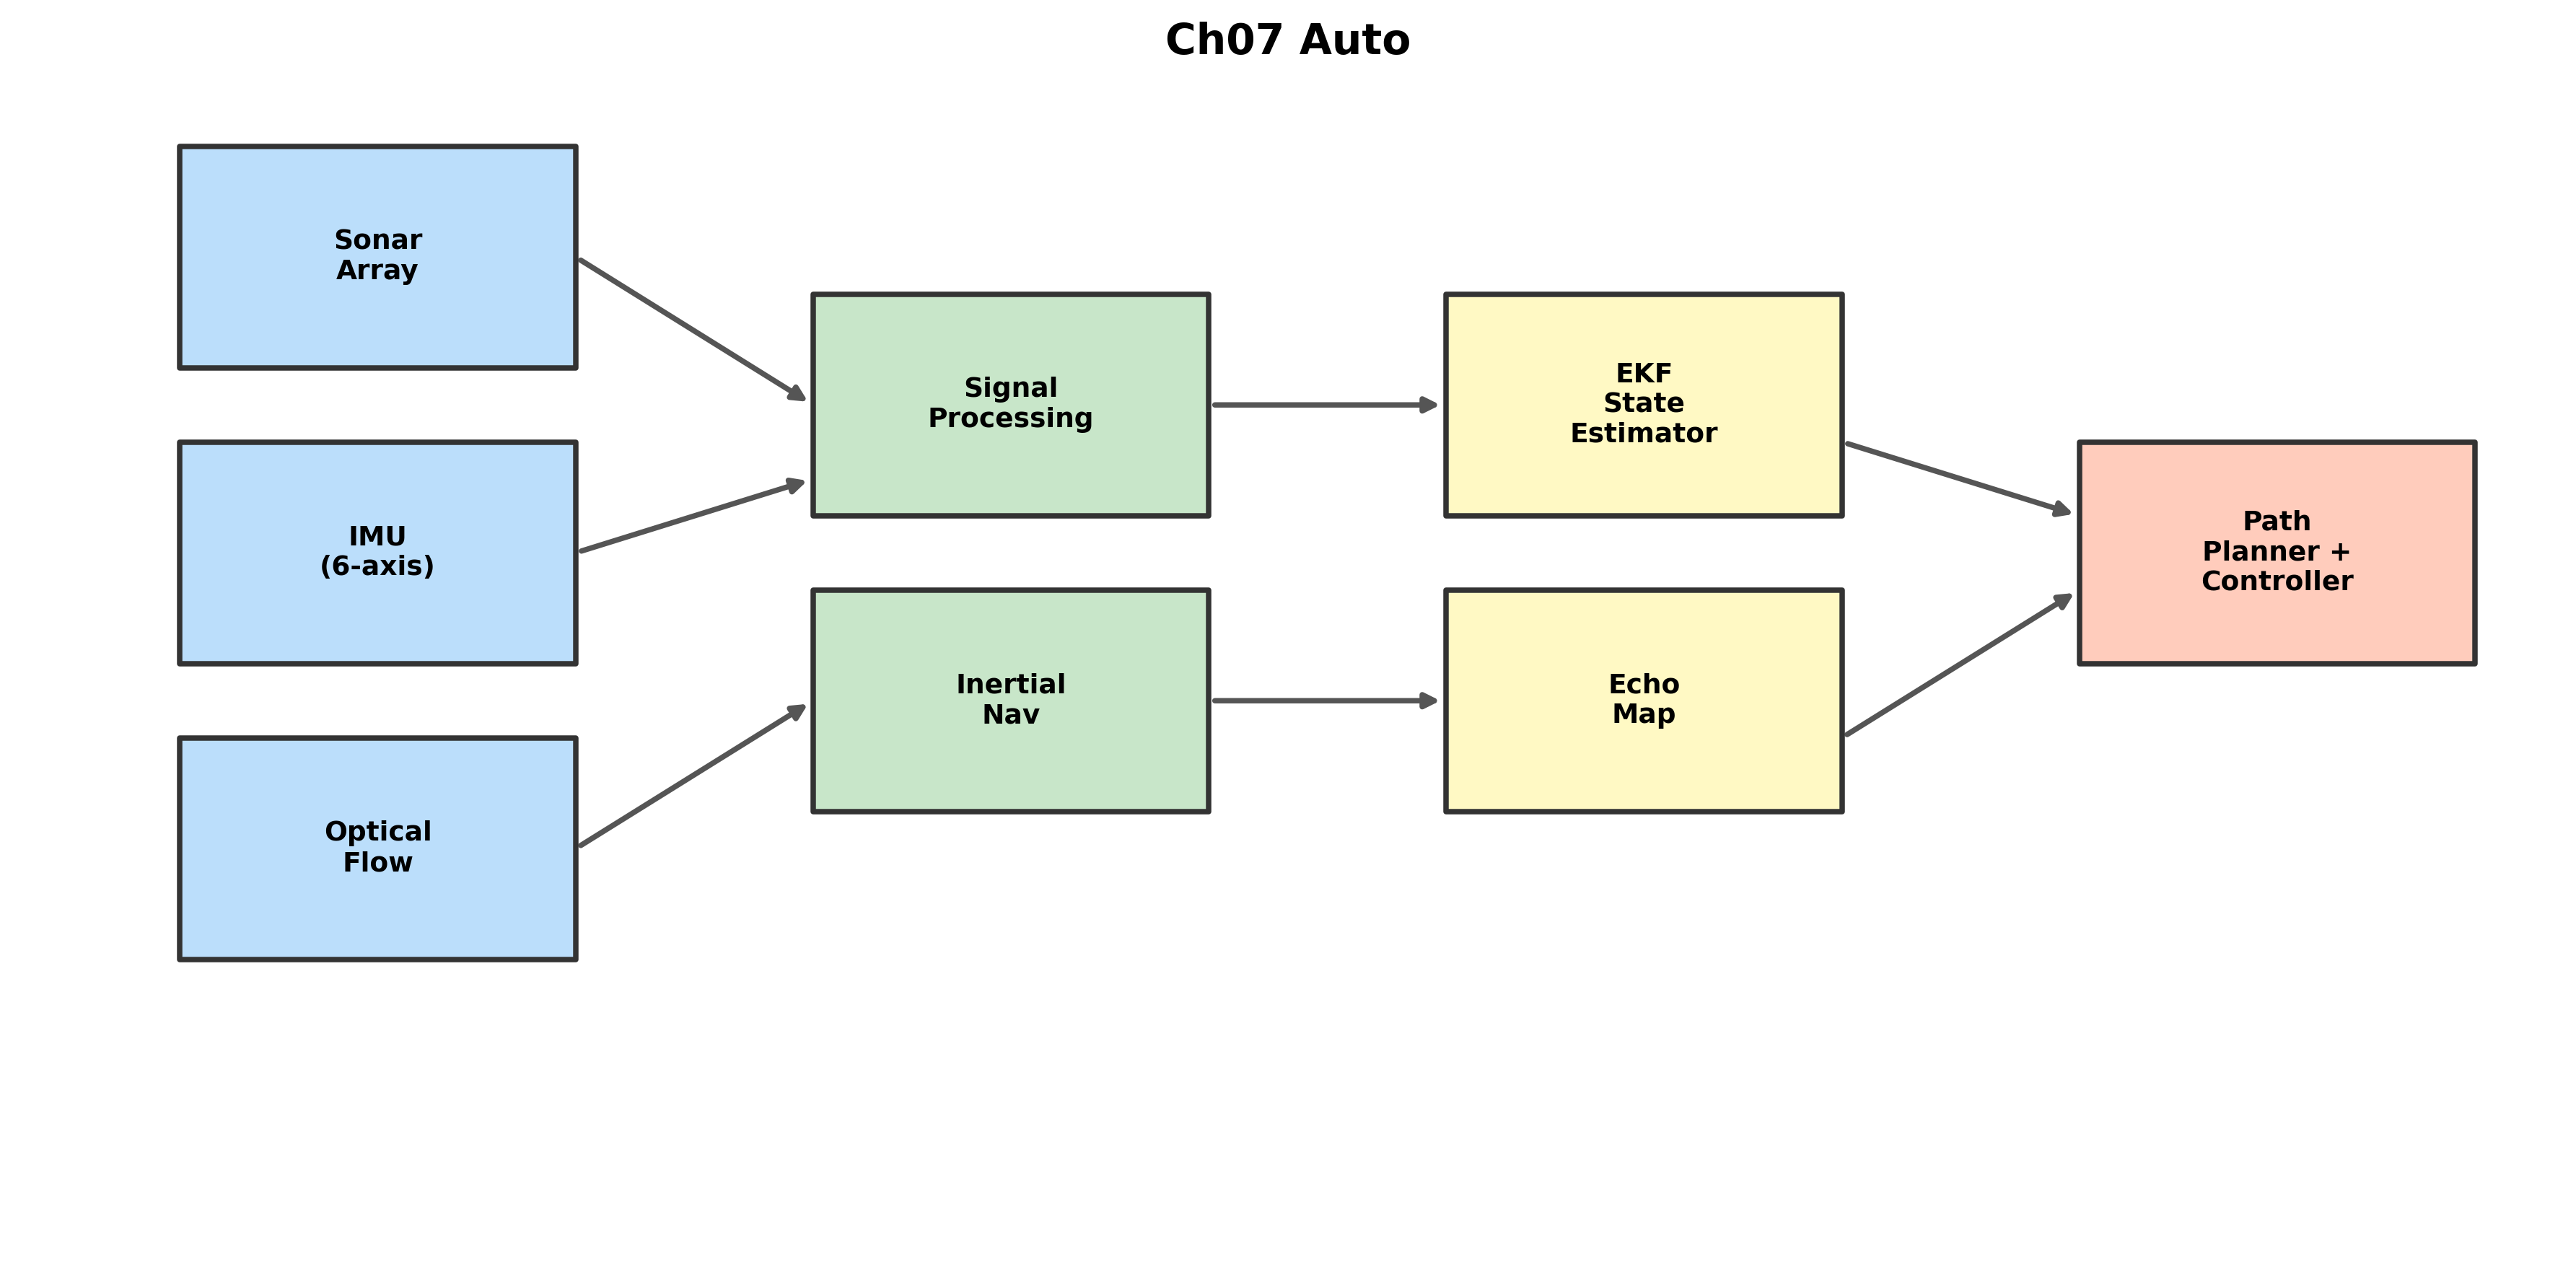
\includegraphics[width=\textwidth]{figures/fig_ch07_auto.png}
    \caption{Stub figure 1 : ch07}
    \label{fig:ch07_1}
\end{figure*}

\en{See} \cite{Thrun2005}\cite{Kalman1960}.
>>>>>>> d28438e746e968070f910361040b7f6540bdd144
